\documentclass[11]{beamer}
\usetheme{Warsaw}
\usepackage[utf8]{inputenc}
\usepackage{amsmath}
\usepackage{amsfonts}
\usepackage{amssymb}
\usepackage{color}
\usepackage{siunitx}
%\usepackage[table]{xcolor} 
\usepackage{color, colortbl}

\definecolor{LightCyan}{rgb}{0.88,1,1}
\definecolor{lightgray}{gray}{0.9}
\usepackage{tikz}
\usetikzlibrary{shapes,snakes,arrows,positioning}


% Define box and box title style
\tikzstyle{mybox} = [draw=red, fill=blue!20, very thick,
    rectangle, rounded corners, inner sep=10pt, inner ysep=20pt]
\tikzstyle{fancytitle} =[fill=red, text=white]



\author{Arindam Basu \hspace{5 cm}\newline{arindam@barc.gov.in}}
\title{Accelerator Technology-Vacuum \newline{Vacuum Introduction Part-2} \newline{Surface Phenomena}}


%\setbeamercovered{transparent} 
%\setbeamertemplate{navigation symbols}{} 
%\logo{} 
%\institute{} 
%\date{} 
%\subject{} 
\begin{document}

\begin{frame}
\titlepage
\end{frame}

%\begin{frame}
%\tableofcontents
%\end{frame}


\begin{frame}{Pumpdown Curve}

\begin{center}
   			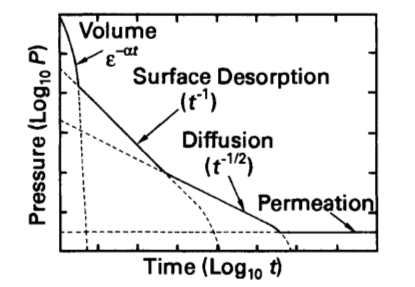
\includegraphics[width=0.5\textwidth]{PD.png}
   			
\end{center}
$P=P_{0}exp(-\dfrac{t}{\tau})  $ is valid for only volume flow. When Surface phenomena is taken into account then 
$P=P_{0}exp(-\dfrac{t}{\tau})+\dfrac{Q_{O}}{S} +\dfrac{Q_{D}}{S} +\dfrac{Q_{P}}{S} $ where $Q_{O},Q_{D},Q_{P}$ are gas throughput by outgassing , diffusion and permeation.
\end{frame}



\begin{frame}{Mono Layer}

\begin{exampleblock}{Monolayer}
A mono layer is the single layer of the molecule on un contaminated solid surface.\break
In a monolayer, solid surface is covered fully with a single layer of molecules.
Monolayer contains approximately $ 7.3 x 10^{14} $ molecules per $cm^2$  for $ N_2 $ \break
A surface exposed to normal atmospheric air have hundred layers of water molecule.
\end{exampleblock}

\begin{exampleblock}{Impingement Rate}
It is the number of Gas molecule collisions with the inner surface of a container. It is also known as particle of Gas moleculae flux density.
It is expressed as $\gamma = \num[round-precision=2,round-mode=figures,scientific-notation=true]{3.5e22} \dfrac{P}{\sqrt{MT}} $ where  $\gamma = $ Impingement Rate in molecules/sec-cm square  $P=$ Pressure in Torr , $M=$Molecular weight of Gas(g/mole) $T=$ Absolute temperature in Kelvin
\end{exampleblock}

\end{frame}



\begin{frame}{Some Important Concepts(contd.}
\begin{exampleblock}{Sticking Probability}
\textbf{Sticking Probability:}Probability with which an impinging molecule will be adsorbed on the surface is the sticking probability.

\textbf{Capture Rate:}It is the number of impinged molecule which is sticking on the container surface or getting captured.\break

\alert{Capture Rate = Impingement Rate x Sticking Probability} 

The pressure, p, exerted on the walls of the vessel depends on  the molecular impingement rate. 
\end{exampleblock}

\begin{exampleblock}{Monolayer Formation Time}
Time $t$ to form mono layer is given by $t=\dfrac{1X10^{-6}}{P}$,  $P$ is in Torr. \break
Thus, for pressures higher than $ 1X10^{-6} $ Torr , surfaces are always covered by at least a monolayer of gas.
\end{exampleblock}


\end{frame}



\begin{frame}{Some Important Concepts}


\begin{exampleblock}{Resident or Sojourn Time}
Resident time is the average time a molecule stays on the surface.It is the function of the molecular weight and the temperature of the surface.
Resident time is can be expressed as De Boer's Formula.

\end{exampleblock}




\begin{exampleblock}{Outgassing And Degassing}
\underline{Outgassing} is the spontaneous evolution of gas from solid or liquid.
Degassing is the deliberate removal of gas from a solid or a liquid.
\end{exampleblock}




\end{frame}










\begin{frame}{Effect of Adsorbed Gas}

\begin{exampleblock}

	\begin{itemize}
		\item 1 monolayer of adsorbed gas influences bonding,wettability, and surface chemical reactions
		\item 1 to 10 monolayers of adsorbed gas affect lubrication and electrical conduction.
		\item 1 to 200 monolayers of adsorbed gas change the absorption of light by a surface.
		\item 200 to 2000 monolayers affect the visual color of surfaces
	\end{itemize}

\end{exampleblock}

\end{frame}

\begin{frame}{Why Vacuum is required}

       \begin{center}
			\includegraphics[width=0.8\textwidth]{WhyVacuumCleanSurface.pdf}
		\end{center}


\end{frame}

\begin{frame}{Use of Vacuum}

      \begin{itemize}
       \item \textbf{Cleanliness:}  low pressure means low number of molecules of potential contaminants.

			\begin{enumerate}
				\item	Extend formation time for native oxides.
				\item	Reduce or eliminate impurities incorporated during processing.
			\end{enumerate}
			
		\item 	\textbf{Plasma generation:}  plasmas can easily be created and sustained in a low pressure environment
used for etching, deposition, and ion implantation.
		\item		\textbf{Lower molecular interference:} Increased mean free path for ions used in sputtering.
		
		
		\item		\textbf{Low friction:} Reduce heat dissipation requirements for processes.
		\item		\textbf{Thermal insulation:} Thermos bottle and Cryogenic systems.

		\item		\textbf{Promote evaporation:} Materials can be evaporated at lower temperatures by reducing the pressure
		\item		\textbf{Mechanical advantage:}Use pressure differences to hold items in place or to transport them from one place to another
      \end{itemize}
      
      

\end{frame}

\begin{frame}{Use of Vacuum}
Two most crucial application of the vacuum
		\begin{itemize}
          \item Semiconductor Fabrication : It requires ultra high vacuum of the order of 10-10 Torr and most stringent quality control.
          \item Drug Manufacture: Medicines are made  under ulta high vacuum condition to avoid any contamination by unwanted molecules.
		
		\end{itemize}

\end{frame}


\begin{frame}{Gas Scattering at a surface}

\begin{exampleblock}{Knudsen's Cosine Law}

\begin{itemize}

\item When a gas molecule strikes a surface it remains on the surface sufficiently long to be fully accommodated

\item Therefore when it leaves the surface, the distribution of velocities follows a cosine law
		
		\begin{center}
			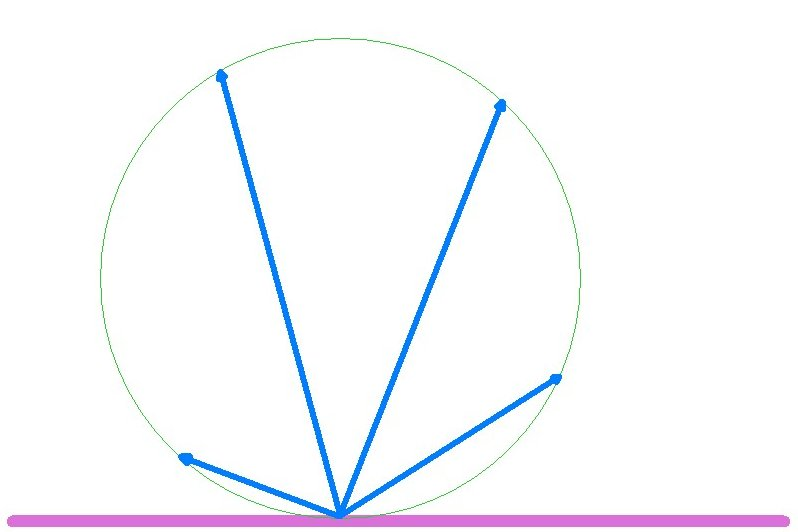
\includegraphics[width=0.2\textwidth]{CosineLawOfScattering.png}
		\end{center}



\end{itemize}


\end{exampleblock}

\end{frame}



\begin{frame}{• Surface Phenomena}

\begin{exampleblock}

\begin{enumerate}
			\item Diffusion.
			\item Permeation.
			\item Evaporation.
			\item Sorption( Adsorption) \& Desorption.
	   	 	\item Chemical Reactions at Solid Surfaces.
			\item Gassing and Degassing of the Surface.
	   	 	
			\item Interaction of charged , neutral particle and photon with surface.
			
	
	\end{enumerate}
\end{exampleblock}


\end{frame}


\begin{frame}{• Surface Phenomena(Contd. )}

\begin{enumerate}
\item DIFFUSION is transport of gas dissolved in the solid to the interior wall of a vacuum system and followed by desorption.
\begin{center}
   			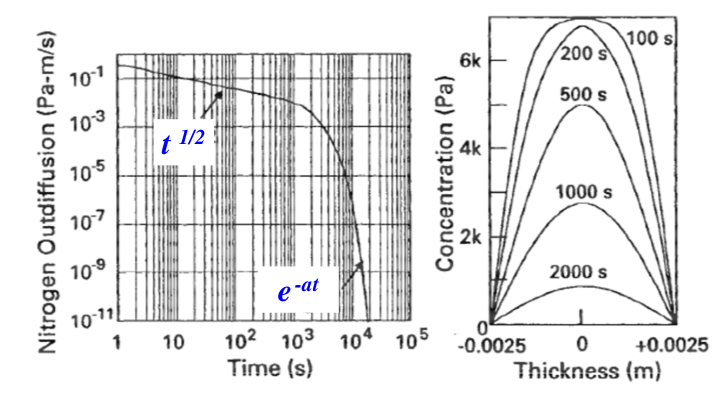
\includegraphics[width=0.5\textwidth]{Diffusion.png}
  	 \end{center}




\end{enumerate}

	


\end{frame}


\begin{frame}{Permeation}
Permeation is the transfer of the fluid through a solid. Permeation is dependent on 
\begin{itemize}
\item Material Combination(Solid and fluid).
\item Temperature ($T$)
\item Thickness($d$)
\item Area ($A$)
\item Pressure Differential.($\Delta P$)
\end{itemize}
Helium is the main gas which tend to enter into the vacuum vessel via glass. Also permeation takes place through O ring.

 \begin{columns}[t]
    
      
   \column{0.5\textwidth}
       \begin{exampleblock}{}
         \begin{center}
			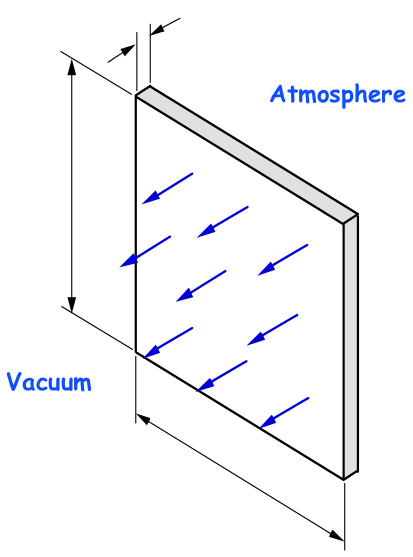
\includegraphics[width=0.3\textwidth]{Permeation.png}
		\end{center}
       \end{exampleblock}
       
    \column{0.5\textwidth}
       \begin{exampleblock}{ }
          \begin{center}
		   $Q_{P}=q_{P}A = \dfrac{K_{P}\Delta P}{A}$ \break
		   Permeation Constant $K_{P}$ has unit $ m^{2}/s $ in SI.		
		\end{center}    
       
       \end{exampleblock}   
   
    \end{columns}   
    
    
   			
  	


\end{frame}


\begin{frame}{Evaporation}

\begin{itemize}
\item Evaporation: when a liquid becomes a gas.
\item Sublimation: when a solid becomes a gas.
\item Vapor: the gas produced when a liquid or solid is evaporated.
\item Condensation: when the vapor becomes a liquid or solid again (condensed phases).
\item Equilibrium: the state of any system in which opposing forces balance each other
\item Volatile: liquids that are easily vaporized -have high vapor pressure.
\item Vapor Pressure:Pressure at which evapouration takes place.
\end{itemize}


\end{frame}


\begin{frame}{Evaporation}

\begin{exampleblock}{Gas load due to Evaporation}
       \begin{center}
			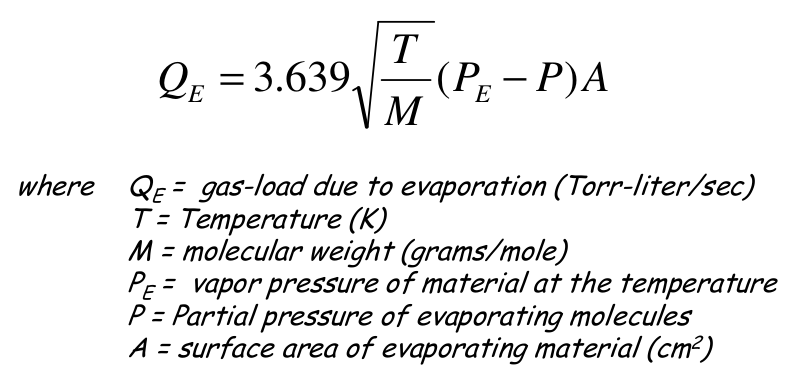
\includegraphics[width=0.8\textwidth]{EvaporationFormula.png}
		\end{center}
Material vapor pressure $P_{E} $ is a strongly dependent on temperature $T$

\end{exampleblock}

\end{frame}

\begin{frame}{Evaporation}

\begin{exampleblock}{Vapor Pressure – Antoine Equation}
       \begin{center}
			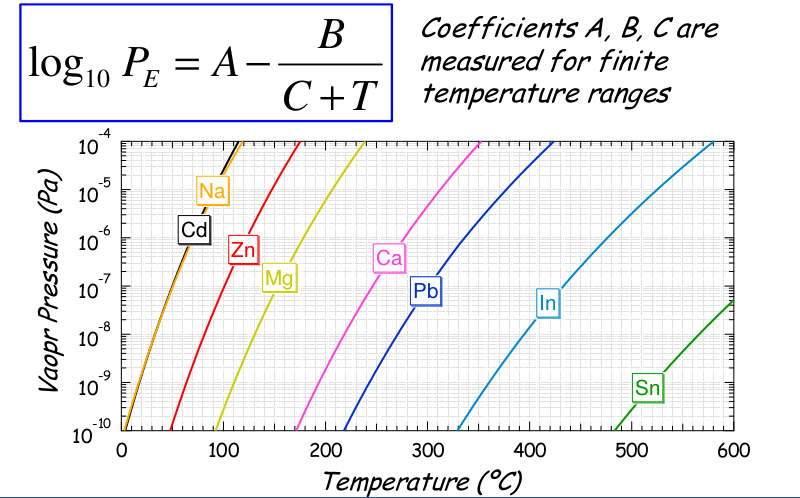
\includegraphics[width=0.8\textwidth]{VaporPrEqn.png}
		\end{center}


\end{exampleblock}

\end{frame}

\begin{frame}{Evaporation}

	\begin{exampleblock}
		
		\begin{itemize}

			\item Certain metals (Cadmium, Zinc, Magnesium) can vaporize in significant quantities at high temperatures of several hundreds of deg C. The use of these metals is therefore avoided in plant construction.
			\item Metals having very low vapor pressure is used as the vacuum construction material.
			\item Natural fibers, in particular,such as paper, contain large quantities of water that escape under vacuum.
			\item \textbf{MORAL:} Vapor pressure must be considered when selecting EVERYTHING that goes into a vacuum system.This includes seals, oil, chamber materials, valves, the wafer, etc.

  		  \end{itemize}

\end{exampleblock}

\end{frame}


\begin{frame}{Sorption and De Sorption}
 SORPTION If a material traps the gas/vapor molecules in its surface then the  process is called sorption.Sorption is the technical name of the gas molecules sticking on the solid surface.\break

Any surface, which is exposed to atmospheric air , have many hundred mono layers of adsorbed molecules on its surface.And most of them are water molecule.  

    \begin{center}
   			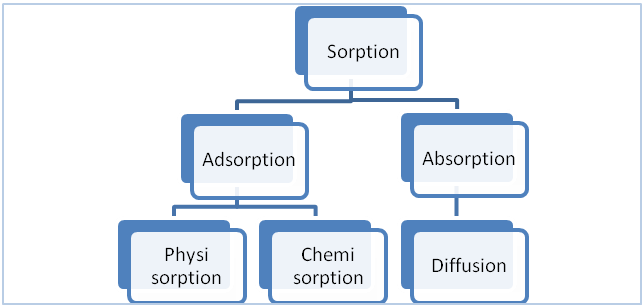
\includegraphics[width=0.5\textwidth]{Sorption.png}
  	 \end{center}

\end{frame}





\begin{frame}{Surface Phenomena-Adsorption}


\begin{exampleblock}{Adsorption}

Adsorption is a process in which molecules are attracted to and become attached to the surface of a solid, resulting in a layer of adsorbed gas being few molecules thick.\\
Adsorption is an attractive force, hence generates heat.\\
Two types of Adsorption:\\

		\begin{center}
 				\begin{itemize}
         			\item Physisorption
					\item Chemisorption
		 		\end{itemize}
		
		\end{center}
	
Another name of chemi sorption is gettering. Materials like Titanium chemically reacts with the gas molecules and absorb them.	   


\end{exampleblock}	


\end{frame}


\begin{frame}{• Surface Phenomena(Contd. )}

   	\begin{center}
   			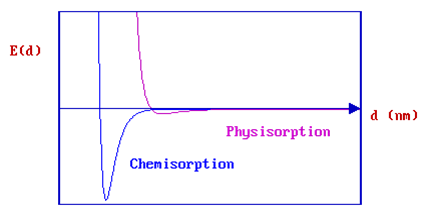
\includegraphics[width=0.2\textwidth]{PhsiChemiSorption.png}
  	 \end{center}
   
   
   \begin{columns}[t]
    
      
   \column{0.5\textwidth}
       \begin{exampleblock}{Chemisorption}
         \begin{itemize}
         	\item Process in which the molecules react chemically to form stable chemical compounds on a solid surface
			\item Characterized by stronger forces and heats of chemisorption are larger ( 250 kcal / mol).
		 \end{itemize}
       \end{exampleblock}
       
    \column{0.5\textwidth}
       \begin{exampleblock}{Physisorption}
         \begin{itemize}
           \item  Process in which the molecules are physically buried in the interstitials of a solid surface.
           \item  Characterized by weak forces and heats of physisorption are small ( 8 kcal / mol).
         \end{itemize}
      
       
       \end{exampleblock}   
   
    \end{columns}



\end{frame}

\begin{frame}{• Adsorption }
\begin{center}
\begin{tabular}{|c|c|}
\hline 
Pressure & $ N_{a}/N_{g} $ \\ 
\hline 
760 & \num[round-precision=2,round-mode=figures,
    scientific-notation=true]{1.5e-5}  \\ 
\hline 
1 & \num[round-precision=2,round-mode=figures,
    scientific-notation=true]{1.1e-2}  \\ 
\hline 
 $ 10^{-3} $ & \num[round-precision=2,round-mode=figures,
    scientific-notation=true]{1.1e1}  \\ 
\hline 
$ 10^{-6} $  & \num[round-precision=2,round-mode=figures,
    scientific-notation=true]{1.1e4}  \\ 
\hline 
$ 10^{-9} $ & \num[round-precision=2,round-mode=figures,
    scientific-notation=true]{1.1e7}  \\ 
\hline 
\end{tabular} 
\end{center}
$ N_{a} $ = Number of gas molecules adsorbed.
$ N_{g} $ = Number of gas molecules in gas state.\\
Gases prone to adsorption are water vapor ($ H_{2}O $ ), Carbon mono oxide ($CO$), Carbon Dioxide($ CO_{2} $) and Oxygen ($ O_{2} $). All these molecules are polar in nature and tend to form Van Der Waal types of bond. Since normal air contains 10 gm of water per meter cube , water is the most abundant adsorbed molecule on a solid surface exposed to atmospheric air.\\
\alert{\textbf{Always break vacuum with dry nitrogen gas.}}  

	
\end{frame}



\begin{frame}{Desorption }

\begin{itemize}
\item Desorption is the release of adsorbed chemical species from the surface of a solid or liquid .
\item Desorption is in equillibrium with sorption in normal atmospheric pressure.
\item In a continously pumped system desorption rate tend to reduce down as with prologed pumping as Contaminated molecular layers on the surface keeps on reducing.
\end{itemize}

\end{frame}



\begin{frame}{• Ways of Desorption }

\begin{itemize}
\item \textbf{Thermal Desorption:} If external thermal energy is added in the system desorption takes place.
\item \textbf{Electron induced De Sorption :}  Electron energy should be greater than  5 ev.
 \item \textbf{Ion induced De Sorption:} Dependent on the energy of the ion. In untreated surface ion discharge cleaning is used to reduce out gassing rate.
 \item \textbf{Photon induced De Sorption :} It is a two step process. Photon produces a photo  electron which actually causes De Sorption.



\end{itemize}

\end{frame}

\begin{frame}{• Thermal Desorption or Baking }

\begin{exampleblock}
   
   \begin{itemize}
   	\item   If temperature increases then thermal de sorption takes place. If this is done intentionally then it is called \textbf{baking.}   

	\item	Adsorb molecules have  lifetimes on the surface given by $\tau=10^{-13}e^{\dfrac{q}{KT}} $ where $q$ is the heat of adsorption.This is  De Boer's Formula.

	\item   kT at room temperature is 1/40 eV.Hence $\tau=10^{-13}e^{40q} $
	
	\item  Mean adsorption stay time  is the avarege lifetimes of an adsorbed molecules ($\tau $)
   \end{itemize}
     
  
  
  
\end{exampleblock}



\end{frame}

\begin{frame}
\begin{center}
    \begin{tabular}{ | l | l | l | }
    \hline
    q(kCal/mole) & T( Kelvin) & Time\\ \hline
   
    10
    & 300
    & \num[round-precision=2,round-mode=figures,
    scientific-notation=true]{2e-6}  Sec (2 $\mu$ Sec)  \\ \hline
	
	
     15
    & 300
    & \num[round-precision=2,round-mode=figures,
    scientific-notation=true]{7e-6}  Sec (7 m Sec)  \\ \hline 
    
    20
    & 300
    & \num[round-precision=2,round-mode=figures,
    scientific-notation=true]{3e1}  Sec (30 Sec)  \\ \hline     
    
    
    25
    & 300
    & \num[round-precision=2,round-mode=figures,
    scientific-notation=true]{1.2e5}  Sec (33 Hr)  \\ \hline   
          
     
    & 600
    & \num[round-precision=2,round-mode=figures,
    scientific-notation=true]{1.1e-4}  Sec (0.11 mSec)  \\ \hline 
    
    30
    & 300
    & \num[round-precision=2,round-mode=figures,
    scientific-notation=true]{5e8} Sec (16 Yr)  \\ \hline   
          
     
    & 600
    & \num[round-precision=2,round-mode=figures,
    scientific-notation=true]{7e-3}  Sec (7 mSec)  \\ \hline     
    
    40
    & 300
    & \num[round-precision=2,round-mode=figures,
    scientific-notation=true]{1e16} Sec (300 Million Yr)  \\ \hline   
          
     
    & 600
    & \num[round-precision=2,round-mode=figures,
    scientific-notation=true]{3e1} Sec (30 Sec)  \\ \hline     
    
    %\hline
    \end{tabular}
\end{center}	

Gases prone to adsorption are water vapor ($ H_{2}O $ ), Carbon Mono Oxide ($CO$), Carbon Dioxide($ CO_{2} $),Oxygen ($ O_{2} $).

\end{frame}








\begin{frame}{• Outgassing Rate}


\begin{exampleblock}{}
Outgassing rate is dependent on:
\begin{enumerate}
		\item Temperature
		\item Surface Finish
		\item Cleanliness
		\item Heat Treatment
		\item Exposure Time
		\item Pumpdown Time

		
\end{enumerate}

\end{exampleblock}		


\end{frame}



\begin{frame}{• Ionization}

\begin{exampleblock}


\begin{enumerate}
		\item Process of formation of Positive or Negative Ions and Free Electrons is called Ionization
\item An atom that loses a single electron is a singly charged Positive Ion
\item An atom that loses multiple electrons is a multiply charged Positive Ion
\item An atom that that is attached with a single electron is a Negative Ion
\item \textbf{Ionization can occur due to charged particle impact, Heat, Radiation.}

		
\end{enumerate}

\end{exampleblock}		


\end{frame}

\begin{frame}{• Electron Impact Ionization}

\begin{exampleblock}

\begin{enumerate}
		\item Electric field $ E = \frac{V}{d}$ .
\item If electron travels a distance $\lambda_{e} $  before colliding with a gas atom/molecule (mean free path,  $\approx \num[round-precision=2,round-mode=figures,scientific-notation=true]{0.5e-6}m$ in atmospheric air), it will gain an energy   $ \frac{U \lambda_{e}}{d} = E \lambda_{e} $
\item The minimum energy to remove the weakest bound electron from its normal state in the neutral atom to a distance beyond its sphere of influence is the Ionization Energy
\item Mean free path for electrons is : $ \lambda_{e} = \frac{4\sqrt{2}}{\lambda_{g}} $  and MFP for ions is : $ \lambda_{i} = \frac{\sqrt{2}}{\lambda_{g}} $ 
where $ \lambda_{g} $  is mean free path for gas 

\item Ionization efficiency of Electron
       \begin{itemize}
        \item This is number of ions produced per unit distance per unit gas pressure

        \item This is a function of electron energy

       
        \item The efficiency is maximum at electron energy of about 100 eV for most of the gases

       
       \end{itemize}
       
		
\end{enumerate}

		
\end{exampleblock}

\end{frame}



\begin{frame}{Paschen's Law}

\begin{exampleblock}

\begin{itemize}
\item Paschen's Law reflects the Townsend breakdown mechanism in gases, that is, a cascading of secondary electrons emitted by collisions in the gap.
\item Electrical breakdown characteristics of a gap are a function (generally not linear) of the product of the gas pressure and the gap length, usually written as, $ V = f(P.d) $
where P is the pressure and d is the gap distance. 
In reality, the pressure should be replaced by the gas density.
\item For air, and gaps on the order of a millimeter, the breakdown is roughly a linear function of the gap length: 
$ V = 30 P d + 1.35 kV $
where d is in centimeters, and p is in atmospheres.

\end{itemize}





\end{exampleblock}





		


\end{frame}




\begin{frame}{Paschen's Curve}
		
	\begin{center}
		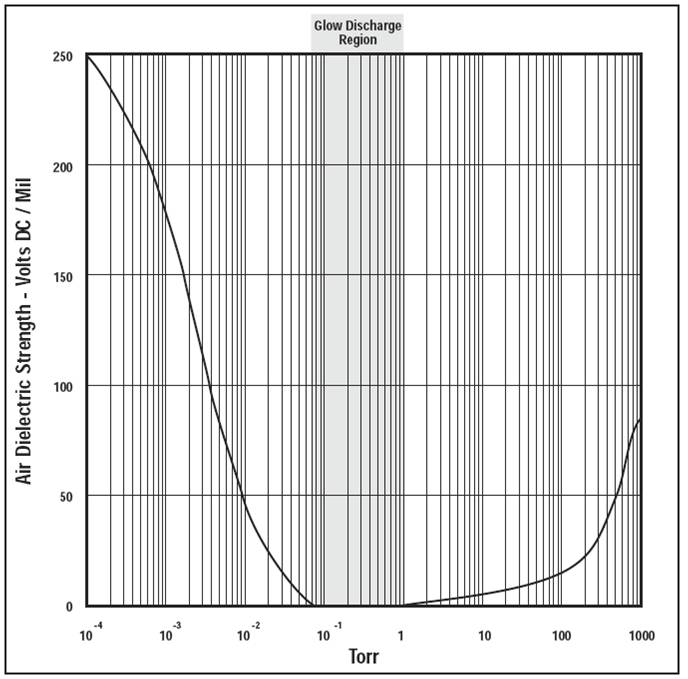
\includegraphics[width=0.8\textwidth]{Dielectric_Breakdown.jpg}	
	\end{center}
	

\end{frame}



\begin{frame}{One Dimensional Pressure Profile}
		
	\begin{itemize}
	\item Since most accelerators and components have one dimension which is
much bigger than the two others (length of the beamlines vs cross-
section of the beampipe), one-dimensional mass-balance equation may
be used: \break
			\begin{center}
             $ V\dfrac{dP(x,t)}{dt}=Q(x,t)-S(x,t)P(x,t)+C(x,t)\dfrac{d^{2}P(x,t)}{dx^2}$
			\end{center}
	
	\item At steady state 
	       \begin{center}
             $ Q(x,t)=S(x,t)P(x,t)-C(x,t)\dfrac{d^{2}P(x,t)}{dx^2}$
			\end{center}
	where S(x), Q(x) are pumping speed and gas load, c(x) is specific gas conductance
	
	
	\end{itemize}
	

\end{frame}


\begin{frame}{One Dimensional Pressure Profile}
		
	
	Consider a simple vacuum system of uniform cross section, with lumped pumps installed every L meters apart, no distributed pumping.
	
	 Let A be the specific surface of the vacuum chamber, in cm squared per meter , and an
uniform thermal outgassing rate, q in mbar l/s cm 2, we have
			
             $ C \dfrac{d^{2}P}{dx^2}=-Aq$
			
	
	 Using boundary condition that  $\dfrac{dP}{dx}=0$ at $x=L/2 $ and $P=\dfrac{AQL}{S}$ at $x=0 $ solution is $ P=\dfrac{AQ}{2C}(Lx-x^{2})+\dfrac{AQL}{S}$
	
	
	
	

\end{frame}


\begin{frame}{One Dimensional Pressure Profile}
		
	
	\begin{center}
		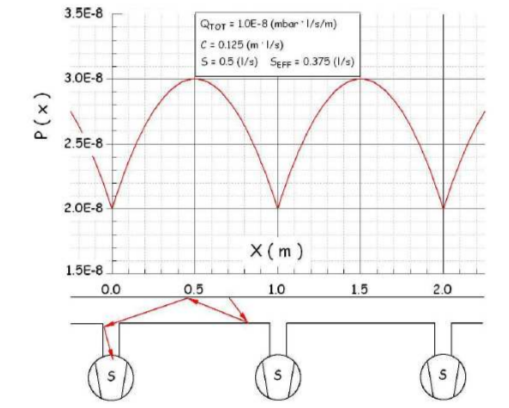
\includegraphics[width=0.8\textwidth]{SpatialPrProfile.png}	
		
	\end{center}
	
	
	
	

\end{frame}


\begin{frame}{One Dimensional Pressure Profile}
		
	
	\begin{center}
		
		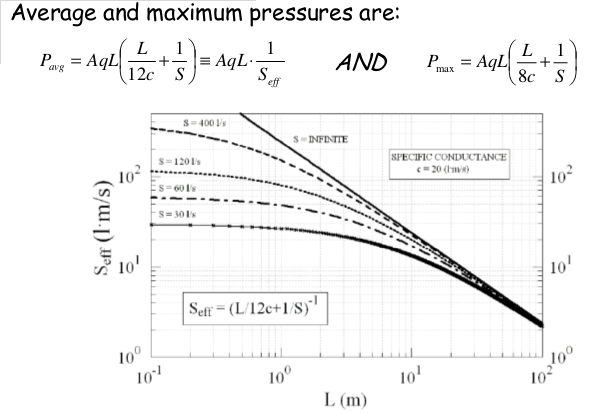
\includegraphics[width=0.8\textwidth]{SpatialPrProfileAvgPr.png}	
	\end{center}
	
	
	
	

\end{frame}









%\begin{frame}
%\begin{thebibliography}{10}
%\bibitem{Goldbach1742}[Goldbach, 1742]
%Christian Goldbach.
%\newblock A problem we should try to solve \break before the ISPN ’43 deadline,
%\newblock \emph{Letter to Leonhard Euler}, 1742.
%\end{thebibliography}

%\begin{block}{Open Questions}
%Is every even number the sum of two primes?
%\cite{Goldbach1742}
%\end{block}
%\end{frame}









\end{document}